% !Mode:: "TeX:UTF-8"
\chapter{Loop Closure}
\label{cpt:11}
\begin{mdframed}  
	\textbf{Goal of Study}
	\begin{enumerate}[labelindent=0em,leftmargin=1.5em]
		\item Understand why loop closure is needed in SLAM.
		\item Understand the principles of the bag-of-words model. 
		\item Use DBoW3 to detect similar images. 
	\end{enumerate}
\end{mdframed}

In this lecture, we will introduce another main module in SLAM: loop closure detection. We know that the primary purpose of SLAM (frontend, backend) is to estimate camera movement. However, the loop closure module is quite different from the previous content, so it is usually considered an independent module. We will introduce the loop detection method in visual SLAM: the bag of words model. And then, we carry out an experiment on the DBoW library so that readers can get a more intuitive understanding.

%\newpage
%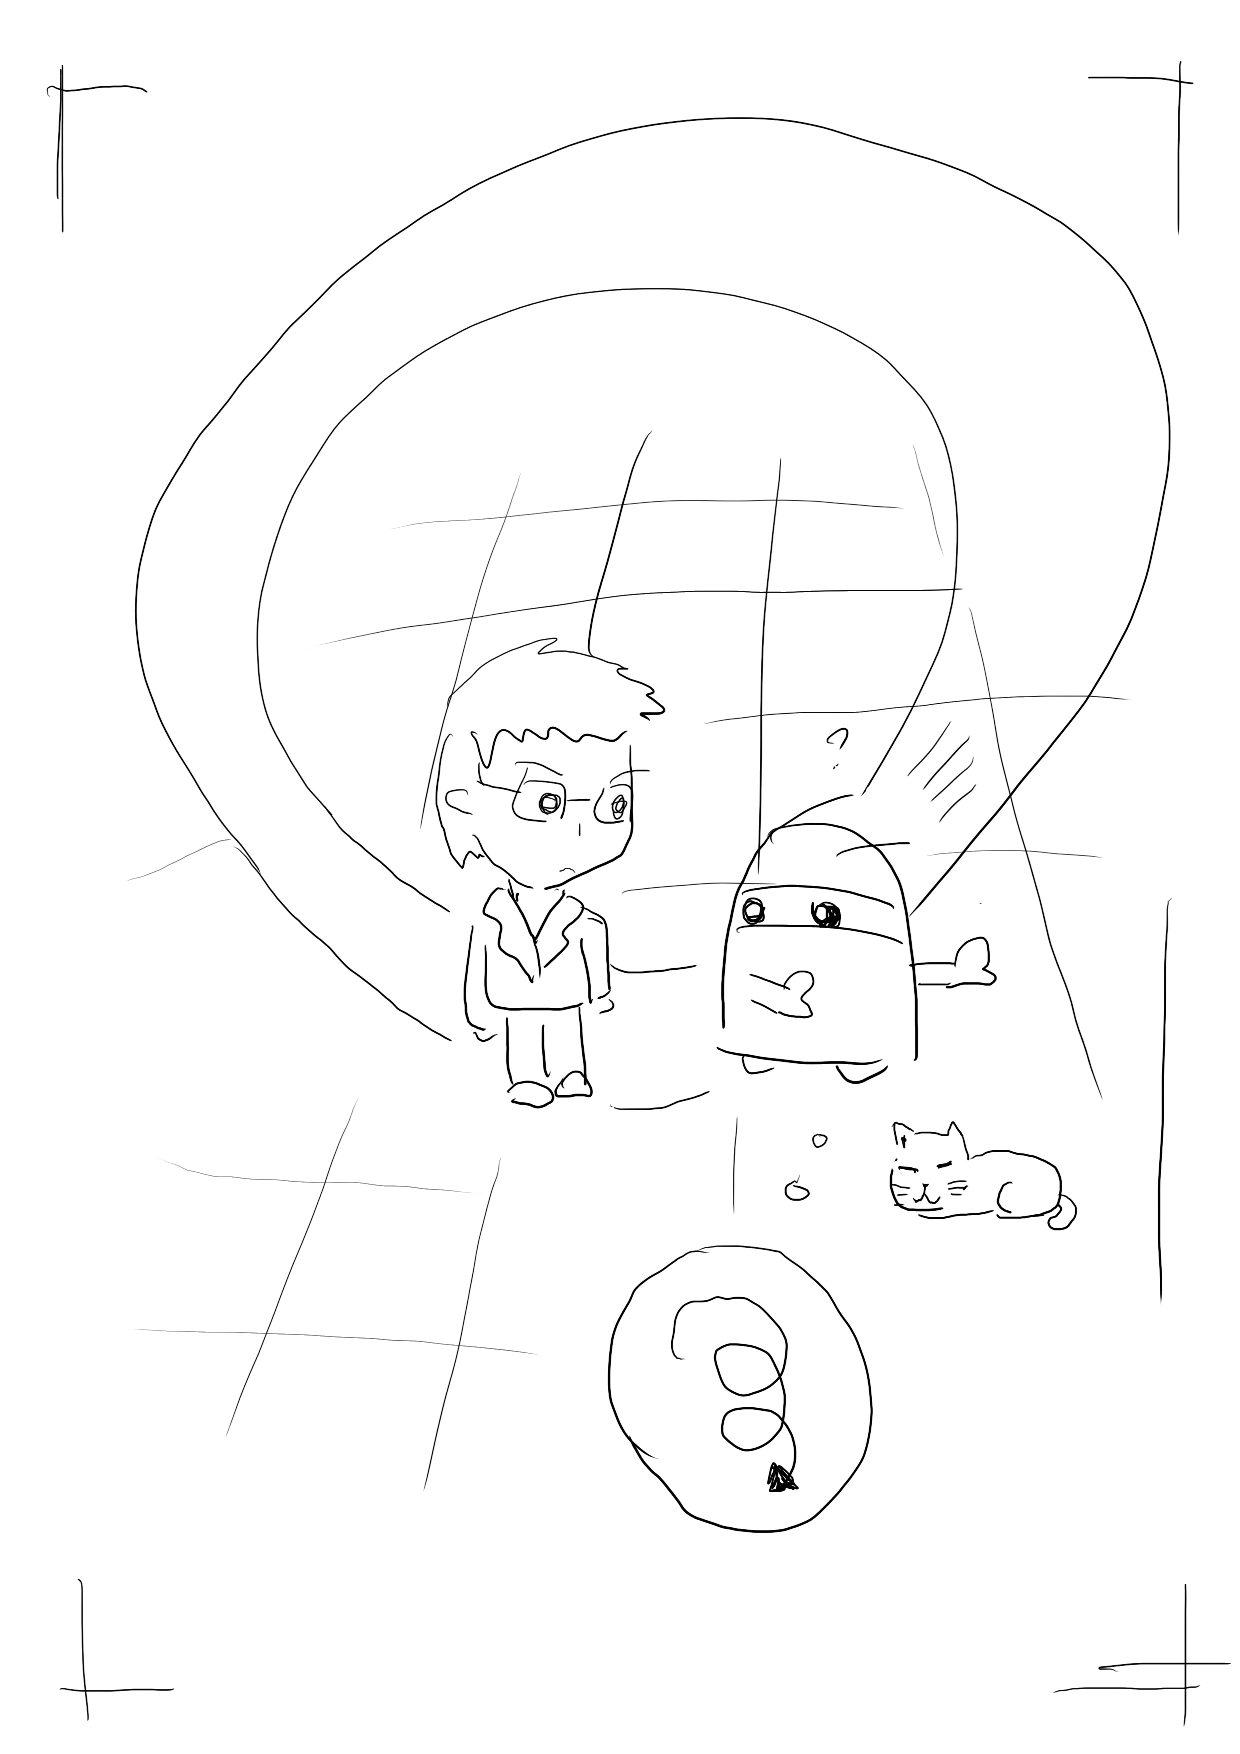
\includepdf{resources/other/ch12.pdf}

\newpage
\section{Loop Closure and Detection}
\subsection{Why Loop Closure is Needed}
We have already introduced the frontend and the backend: the frontend provides short-time trajectory/landmarks estimation and the map's initial value. The backend is responsible for optimizing all these data. However, if we only consider the adjacent keyframes like VO, then the errors will inevitably accumulate with time so that the entire SLAM will suffer from the accumulative error. The result of long-term estimation will not be reliable. In other words, we cannot construct \textit{globally consistent} trajectories and maps.

Let's take an example. In the map-building stage of autonomous driving, we usually designate the collection vehicle to circle several times in a given area to cover all the collection areas. Suppose we extract the features at the frontend, then ignore the feature points, and use a pose graph to optimize the entire trajectory at the backend, as shown in \autoref{fig:drift}(a)~. Since the frontend gives only sequential pose constraints, for example, it may be $\mathbf{x}_1-\mathbf{x}_2, \mathbf{x}_2-\mathbf{x}_3$, etc. However, due to the error in the estimation of $\mathbf{x}_1$, $\mathbf{x}_2$ is determined according to $\mathbf{x}_1$, $\mathbf{x}_3$ is again determined by $ \mathbf{x}_2$. By analogy, errors will be accumulated, making the result of backend optimization look like what is shown in \autoref{fig:drift}~(b), which gradually tends to be inaccurate. In this application scenario, we should use the loop closure information to determine that the vehicle reaches the same place when we pass the same road.

\begin{figure}[!htp]
	\centering
	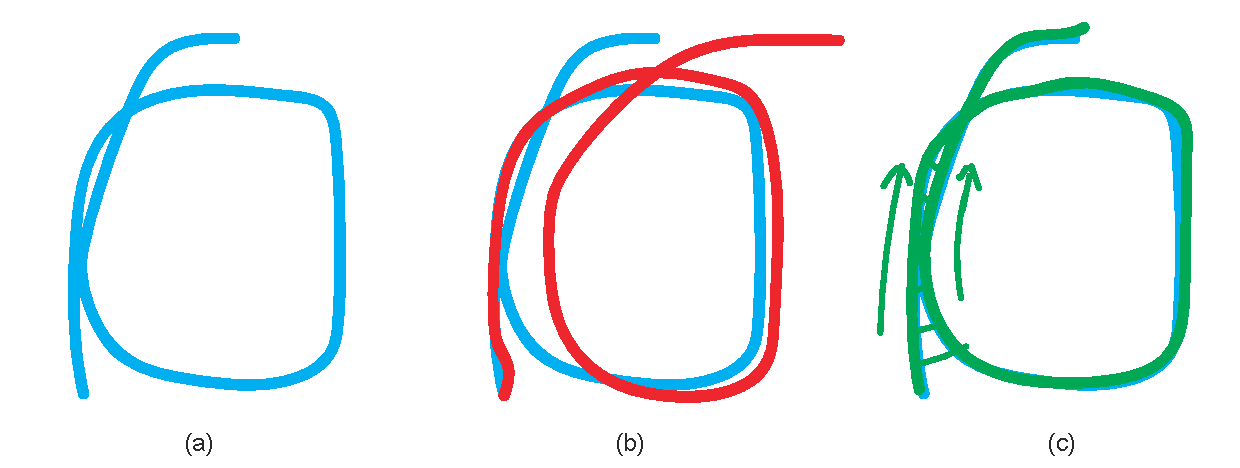
\includegraphics[width=0.8\textwidth]{loopclosure/illustrate-loop.pdf}
	\caption{Accumulated drift. (a) Real trajectory. (b) Accumulated error if we only consider adjacent keyframes. (c) Add loop closure to reduce the accumulated drift. }
	\label{fig:drift}
\end{figure}

Although the backend can estimate the maximum posterior error, it depends on the BA or the pose graph's structure. If there are only adjacent keyframe constraints, we cannot do much, nor can we eliminate the accumulated error. However, the loop closure detection module can provide constraints on longer time other than just adjacent frames: for example, the pose constraint between $\mathbf{x}_1-\mathbf{x}_{100}$. Why do we want to constrain those keyframes? Because we noticed that the camera returns to a previously visited scene, and it acquires similar data ln history. The key to loop detection is how to detect this fact effectively. If we can successfully see this, we can provide more valid constraints for the backend pose graph to get a better estimate, especially a globally consistent estimate. Since the pose graph can be regarded as a point-spring system, loop detection is equivalent to adding additional springs to the graph, which improves the system's stability. The reader can also intuitively imagine that the loop edge ``pulls'' the edge with accumulated error back to the correct position-if the loop itself is right.


Loop detection is of great significance to SLAM systems. It is related to the correctness of our estimated trajectory and map in a long time. On the other hand, since loop detection provides the correlation between current data and historical data, we can also use loop detection for relocation. Relocation is also beneficial in most applications. For example, if we record a track for a scene in advance and build a map, we can let the robot follow this track for navigation, and relocation can help us determine our position on this track. Therefore, the loop detection improves the accuracy and robustness of the entire SLAM system. In some cases, we call a system with only a frontend and a local backend as \textit{VO} and call a system with loop closing and a global backend as \textit{SLAM}.

\subsection{How to Close the Loops}
Let's consider how to implement loop detection. There are several different ways of thinking about this problem, including theoretical and engineering.


The simplest way is to perform feature matching on any image pairs and determine which of them are related according to the number of correct matches. This is indeed a simple and effective idea. The disadvantage is that we blindly assume that ``any two images may have loops,'' which makes the number of detection too large: for $N$ possible loops, we have to detect $C_N^2$ times. It has the complexity of $O(N^2)$, which grows too fast as the trajectory becomes longer and is not practical in most real-time systems. Another simple way is to extract historical data and perform loop detection randomly. For example, randomly select five frames among $n$ frames and compare them with the current frame. This approach can maintain a constant time calculation, but when the number of frames $N$ increases, the probability of drawing a loop is significantly reduced, making the detection efficiency low.

The simple ideas mentioned above are too coarse. Although random detection is indeed useful in some implementations like {\cite{Endres2014}}, we at least hope that there is a prediction of ``there may be a loop somewhere'' so that the detection is not so blind. Such approaches can be roughly divided into two ideas: odometry-based or appearance-based. Based on the geometric relationship, when we find that the current camera moves close to a certain position before, we detect whether they have a loop relationship~\cite{Hahnel2003}. This is naturally an intuitive idea, but it is hard to estimate the accumulated drift amount unless we have global position measurements like GPS. Therefore, this approach has a logical problem because loop detection aims to eliminate accumulated errors. But the odometry-based approach assumes that "the accumulated error is small so that the loop can be detected." If the assumption does not hold, such methods cannot work when the cumulative error is large~\cite{Beeson2010}.

The other method is based on appearance. It has nothing to do with the estimation of the frontend or the backend and only determines the loop detection relationship based on the two images' similarity. This approach eliminates accumulated errors and makes the loop detection module a relatively independent module in the SLAM system (of course, the frontend can provide the extracted feature points). Since it was proposed in the early 21st century, the appearance-based loop detection method can effectively work in different scenarios and has become the mainstream method in visual SLAM and applied to the actual system {\cite{Ulrich2000, Latif2013, Mur-Artal2015}}.

In the appearance-based loop detection algorithm, the core problem is how to calculate the similarity between images. For example, for image $\mathbf{A}$ and image $\mathbf{B}$, we need to design a method to calculate the similarity score between them: $s(\mathbf{A}, \mathbf{B })$. Of course, this score will take a value in a certain interval, and when it is greater than a certain amount, we think that there is a loop. Readers may have questions: Is it difficult to calculate the similarity between two images? For example, intuitively, an image can be expressed as a matrix, so how about subtracting two images directly and then taking a certain norm?

\begin{equation}
	s(\mathbf{A}, \mathbf{B}) = \| \mathbf{A}-\mathbf{B} \|.
\end{equation}

Why don't we do this?

\begin{enumerate}
	\item As mentioned earlier, the pixel grayscale is an unstable measurement value, which is severely affected by the ambient light and camera exposure. Assuming that the camera is not moving and we turn on an electric light, the image will be brighter overall. In this way, even for the same data, we will get a significant difference value.
	\item On the other hand, when the camera's viewing angle changes a little, even if each object's luminosity does not change, their pixels will be transformed in the image, resulting in a large difference in value.
\end{enumerate}

Due to the existence of these two situations, in practice, even for very similar images, $\mathbf{A}-\mathbf{B}$ will often get an (unrealistic) enormous value. So we say that this function {cannot reflect the similar relationship between images}. It involves a definition of ``good'' and ``bad.'' We have to ask, what kind of function can better reflect the similar relationship, and what kind of function is not good enough? From here, two concepts can be drawn: \textit{perceptual aliasing} and \textit{perceptual variability}. Let's discuss it in more detail now.

\subsection{Precision and Recall}
From a human point of view (at least we think), we can feel that ``the two images are similar'' or ``the two photos were taken from the same place'' with high accuracy. But since we have not yet grasped the human brain's working principle, we cannot clearly describe how we accomplish this. From a program point of view, we hope that algorithms can reach judgments consistent with humans or facts. When we feel that the two images were taken from the same place, we expect the loop detection algorithm to result as ``this is a loop.'' Conversely, if we think that the two images were taken from different places, the program should also judge that ``this is not a loop.'' Readers with a machine learning background should feel how similar this passage is to machine learning.  Of course, the judgment of the algorithm is not always consistent with our human thinking, so there may be four situations in \autoref{table:loopclosure}~:

\begin{table}[!htp]
	\centering
	\caption{Classification of the loop detection results}
	\label{table:loopclosure}
	\begin{tabu}{c|c|c}
		\toprule
		Algorithm $\backslash$ Fact & Is loop & Not loop\\ 
		\midrule
		Is loop & True Positive & False Positive \\ 
		Not loop & False Negative & True Negative\\ 
		\bottomrule
	\end{tabu} 
\end{table}

The term negative/positive come from medical terms. False-positive is also called perceptual bias, and false negative is called perceptual variation (see \autoref{fig:FPandFN}). For the convenience of writing, we use the abbreviation TP for true-positive, and FN for false-negative, etc. Since we want the algorithm to be consistent with human judgment, we hope that TP and TN should be as high as possible, and FP and FN should be as low as possible. Therefore, for a particular algorithm, we can count the number of occurrences of TP, TN, FP, and FN on a certain dataset and calculate two statistics: \textit{accuracy rate} and \textit{recall rate} (precision \& recall)
\begin{equation}
	\mathrm{Precision} = \mathrm{TP}/(\mathrm{TP}+\mathrm{FP}), \quad \mathrm{Recall} = \mathrm{TP}/(\mathrm{TP}+\mathrm{FN}).
\end{equation}

\begin{figure}[!htp]
	\centering
	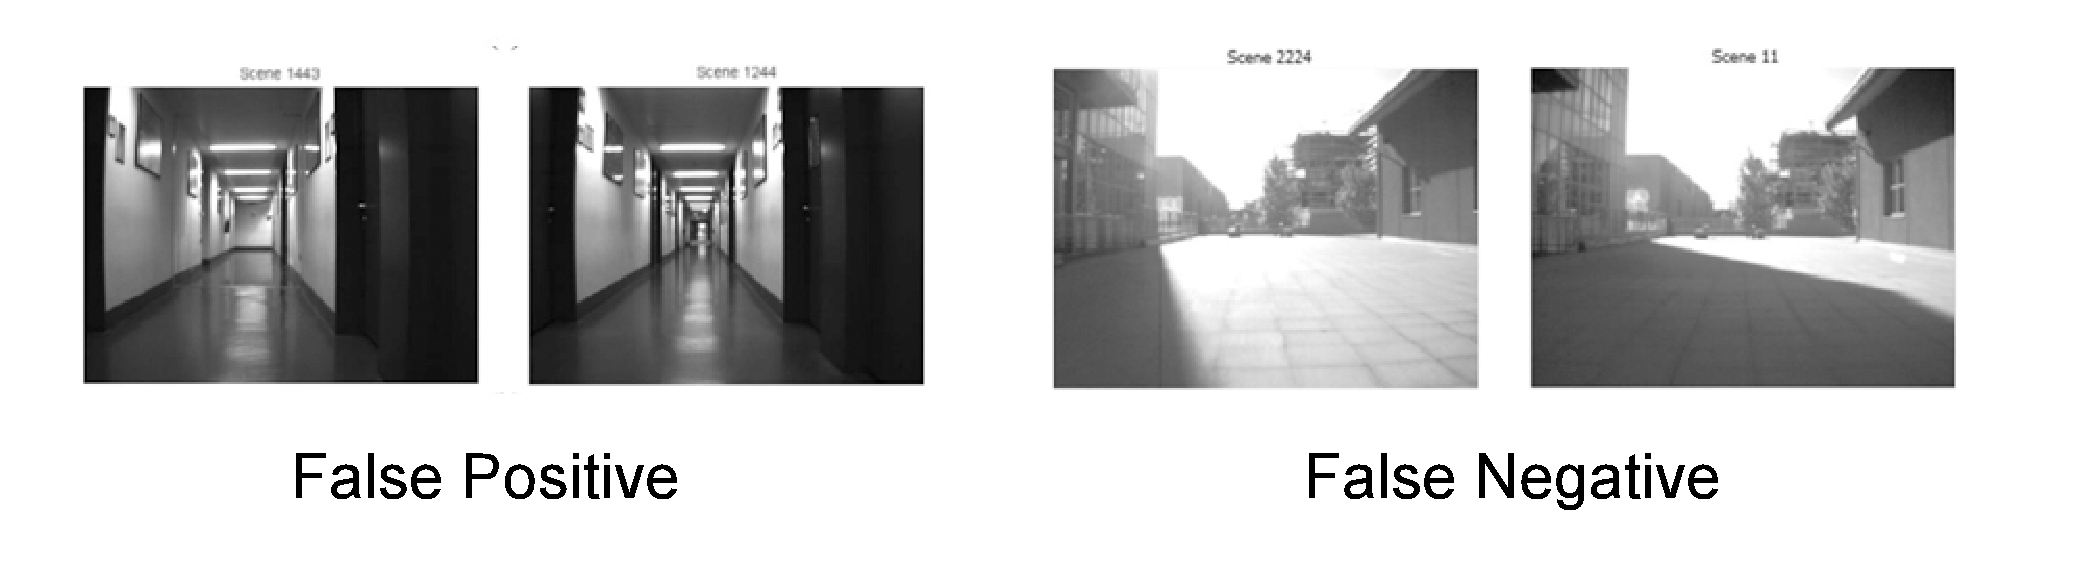
\includegraphics[width=0.9\textwidth]{loopclosure/FPandFN}
	\caption{Example of false-positive and false-negative scenes. Left: the images look the same but actually taken from different spaces. Right: the images are from the same place, but the appearance is different.}
	\label{fig:FPandFN}
\end{figure}

Literally, the accuracy rate describes the probability that all the loops extracted by the algorithm are indeed true loops. The recall rate refers to the probability of loops being detected from all real loops. Why shall we take these two statistics instead of one? Because they are usually a pair of contradictions.

An algorithm often has many setting parameters. For example, when a certain threshold is raised, the algorithm may become more ``strict''. It detects fewer loops and improves accuracy. But at the same time, because the number of detection has decreased, many real loops may be missed, resulting in a decline in the recall rate. Conversely, if we choose a more relaxed configuration, the number of detected loops will increase, resulting in a higher recall rate. But there may be incorrectly detected loops so that the accuracy rate will decrease.

In order to evaluate the quality of the algorithm, we will test its $P$ and $R$ values under various configurations and then make a precision-recall curve (see \autoref{fig:PRCurve}). When using the recall rate on the horizontal axis and the accuracy rate on the vertical axis, we will care about the degree to which the entire curve deviates to the upper right, the recall rate at 100\% accuracy, or the accuracy at 50\% recall rate, as evaluation indicators. However, please note that we usually cannot say that algorithm A is better than algorithm B in general. We may say that A has a good recall rate when the accuracy rate is high, while B can guarantee a good accuracy rate when the recall rate is 70\%, and so on.

\begin{figure}[!ht]
	\centering
	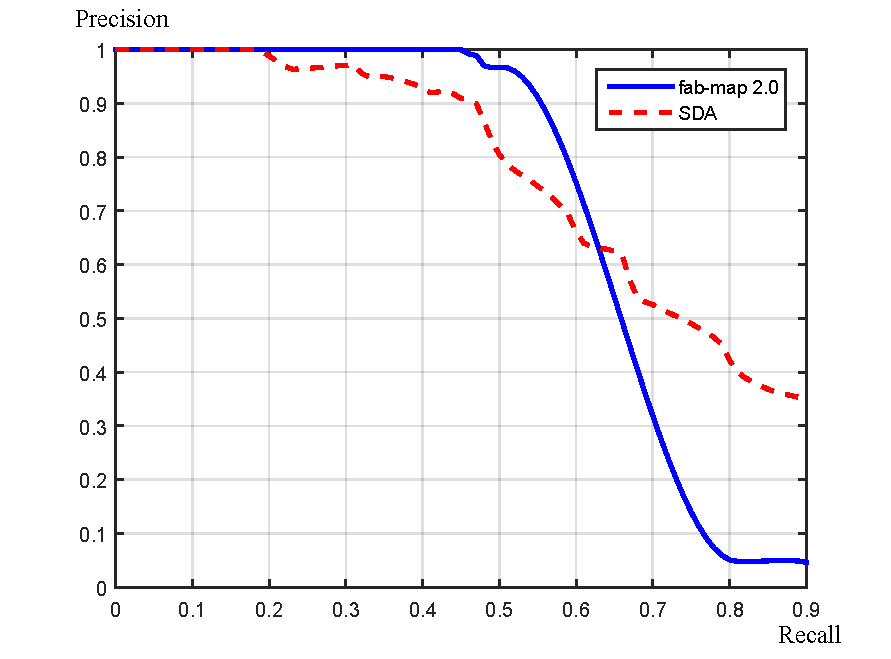
\includegraphics[width=0.66\textwidth]{loopclosure/prcurve}
	\caption{Example of the precision-recall curve {\cite{Gao2015b}}. As the recall rate increases, the detection conditions become looser, and the accuracy rate decreases. A good algorithm can still guarantee a better accuracy rate in a high recall rate.}
	\label{fig:PRCurve}
\end{figure}

It is worth mentioning that we have higher requirements for accuracy in SLAM while being relatively tolerant to the recall. The false-positive loops will add fundamentally wrong edges to the backend pose graph, sometimes causing the optimization algorithm to give completely wrong results. Imagine if the SLAM mistakenly treats all the desks as the same one. What will happen to the created map? You may see that the corridor is not straight, the walls are staggered, and finally, the entire map is invalid. In contrast, if the recall rate is lower, some loops are probably not detected, and the map may be affected by some accumulated errors, but the other loops may eliminate them. Therefore, when choosing the loop detection algorithm, we are more inclined to set the parameters more strictly or add the step of \textit{loop verification} after the detection.

So, back to the previous question, why not use $\mathbf{A}-\mathbf{B}$ to calculate similarity? We will find that its accuracy and recall are inferior to most current methods, and there may be many false-positive or false-negative cases, so it is ``not good.'' So, which method is better?

\section{Bag of Words}
Since directly subtracting two images is not good enough, then we need a more reliable method. Recalling the previous lectures' content, we may have an intuitive idea: Why not use VO feature points to detect the loops? We may match the feature points of the two images just like VO. Furthermore, according to the feature matching, we can also calculate the motion between the two images. Of course, there are some problems with this approach. For example, feature matching will be time-consuming, feature description may be unstable when the illumination changes, etc. But it is very close to the bag of words we will introduce. Let's talk about the bag of words first and then discuss the implementation details.

The purpose of Bag-of-Words (BoW) is to describe an image in terms of ``what kinds of features are there on the image.'' For example, we say a person and a car in one photo; and two people and a dog in another photo. According to this description, the similarity of the two images can be measured. To be more specific, we need to do the following things:

\begin{enumerate}
	\item Determine the concepts of people, cars, and dogs-corresponding to the word. Many words are put together to form a dictionary.
	\item Detect which predefined words in the dictionary appear in an image-we use the appearance of words (histogram) to describe the entire image. In this way, we convert an image into a vector description.
	\item Compute the similarity by the histogram in the second step.
\end{enumerate}

Let's give an example. Assume we get a dictionary in some way. There are many words recorded in the dictionary, and each word has a certain meaning. For example, \textit{person}, \textit{car}, and \textit{dog} are all words recorded in the dictionary. We might as well write them as $w_1, w_2, w_3$. Then, for any image A, according to the words they contain, it can be written as:
\begin{equation}
	A = 1 \cdot w_1+1\cdot w_2 + 0 \cdot w_3.
\end{equation}

Since the dictionary is fixed, we may use the vector $[1,1,0]^\mathrm{T}$ to express the meaning of $A$. Through dictionaries and words, only one vector can describe the entire image. This vector represents the information of "whether the image contains a certain type of feature," which is more stable than the pure gray value. And because the description vector is only about the existence of the words rather than their order, it has nothing to do with the object's spatial position and arrangement order. Therefore, when the camera moves a little, as long as the object is still appearing in the field of vision, we can guarantee that the description vector does not change \footnote{Although this property sometimes brings some problems, for example, is the face with the eyes under the mouth still a human face? }. Based on this feature, we call it Bag-of-Words instead of List-of-Words. The emphasis is on the presence or absence of Words, regardless of their order. Therefore, it can be said that a dictionary is similar to a collection of words.

Going back to the above example, in the same way, the vector $[2,0,1]^\mathrm{T}$ can describe the image $B$. If you only consider ``whether it appears'' without considering the quantity, it can also be $[1,0,1]^\mathrm{T}$. At this time, this vector is binary. Therefore, by designing a particular calculation method based on these two vectors, the similarity between the images can be determined. Of course, if there are still some different ways to calculate the difference between two vectors, for example, for $\mathbf{a}, \mathbf{b} \in \mathbb{R}^W$, we can calculate:
\begin{equation}
	s\left( {\mathbf{a},\mathbf{b}} \right) = 1 - \frac{1}{W}\left\| {\mathbf{a} - \mathbf{b}} \right\|_1,
\end{equation}
where we take the $\mathcal{L}_1$ norm, which is the sum of the absolute values of the elements. Please note that when the two vectors are exactly the same, we will get 1; when the two vectors are completely different (where $\mathbf{a}$ is 0, $\mathbf{b}$ is 1), we will get 0. This defines the similarity of the two description vectors and establishes the similarity between the images.

Yes, what's next?
\begin{enumerate}
	\item Where does the dictionary come from?
	\item If we can calculate the similarity score between two images, is it enough to close the loop?
\end{enumerate}

Next, we first introduce the dictionary's generation method and then present how to use the dictionary to calculate the similarity between two images.

\section{Train the Dictionary}
\subsection{The Structure of Dictionary}
According to the previous introduction, the dictionary is composed of many words, and each word represents a concept. A word is different from a single feature point. It is not extracted from a single image but a combination of a specific type of feature. Therefore, the dictionary generation problem is similar to a clustering problem.

Clustering is a widespread approach in unsupervised machine learning, which lets the machine find the data structure by itself. Training BoW's dictionary is also one of them. First, suppose we have extracted feature points from many, let's say $N$, images. Now, we want to find a dictionary with $k$ words. Each word can be regarded as a collection of local adjacent feature points. We can solve this with the classic K-means (K-means) algorithm {\cite{Lloyd1982}}.

K-means is a straightforward and effective method. It is widely used in unsupervised learning, and we briefly introduce its principles below. Let's say there are $N$ data, and you want to classify them into $k$ categories, then using K-means to do it mainly includes the following steps:

\begin{mdframed}
	\begin{enumerate}
		\item Randomly select $k$ centers: $c_1, \cdots, c_k$.
		\item Compute the distance between each data sample to the cluster centers. Assign the closest cluster to this sample. 
		\item Re-compute the centers of the clusters. 
		\item If the centers converge, exit. Otherwise, return to step 2. 
	\end{enumerate}
\end{mdframed}

The K-means approach is simple and effective, but there are some problems, such as the need to specify the number of clusters, randomly select the center point so that each clustering result is different, and some efficiency issues. Later, researchers also developed algorithms such as hierarchical clustering, K-means++{\cite{Arthur2007}} to make up for its shortcomings, but these are all later improvements. We will not discuss them in detail. In short, according to K-means, we can cluster a large number of feature points that have been extracted into a dictionary containing $k$ words. The question now becomes how to find the dictionary's corresponding word based on a specific feature point in the image.

There is still a simple idea: just compare each word and choose the most similar word-this is, of course, a practical approach. However, considering the versatility of the dictionary\footnote{Would you call a page of paper with only ten words a dictionary? I believe that most people's dictionaries are quite heavy. }, we usually use a larger-scale dictionary to ensure that the image features in the current environment have all appeared in the dictionary or have similar expressions. If you think it's not a hassle to compare ten words one by one, how about ten thousand? How about one hundred thousand?

If readers have learned data structure before, this $O(n)$ search algorithm is obviously not what we want. If the dictionary is sorted, then the binary search can improve search efficiency and reach the logarithmic level of complexity. In practice, we may use more complex data structures, such as the Chou-Liu tree {\cite{Chow1968}} in Fabmap {\cite{Cummins2008, Cummins2010, Cummins2011}}. But we don't want to write this book as a collection of complex details, so we introduce another simpler and more practical tree structure {\cite{Galvez-Lopez2012}}.

In the document of~\cite{Galvez-Lopez2012}, a k-d tree is used to express the dictionary. Its idea is straightforward (as shown in \autoref{fig:lp-dict}), similar to hierarchical clustering, and a direct extension of k-means. Suppose we have $N$ feature points, and we want to build a tree with a depth of $d$ and $k$ forks, then the approach is as follows\footnote{We used $k$ and $d$ to express the branches of the tree, and the depth, which may remind you about the k-d tree~\cite{Bentley1975}. Although the practices are different, the meanings they express are indeed the same. }:

\begin{mdframed}
	\begin{enumerate}
		\item At the root node, use k-means to cluster all samples into $k$ classes (in practice, k-means++ is used to ensure clustering uniformity). This gives the first layer.
		\item For each node in the first layer, gather the samples belonging to that node into the $k$ class to get the next layer.
		\item Repeat the second step until the leaf layer. The leaf layer is the so-called \textit{words}.
	\end{enumerate}
\end{mdframed}

\begin{figure}[!ht]
	\centering
	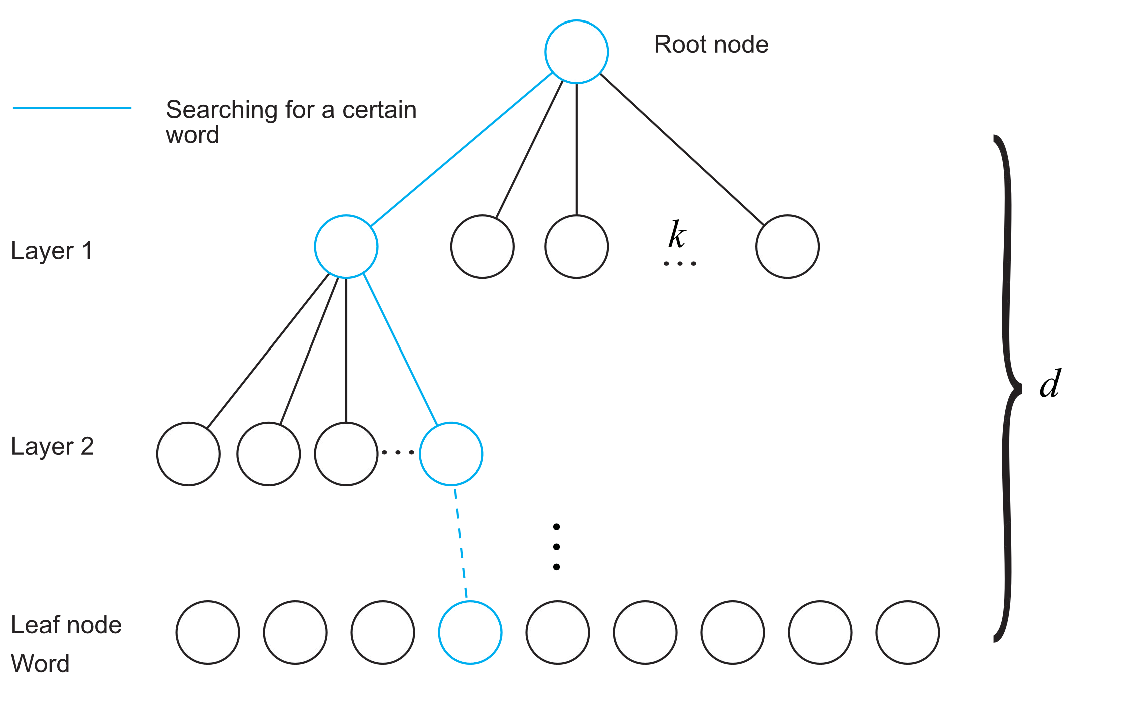
\includegraphics[width=0.9\textwidth]{loopclosure/dict}
	\caption{Schematic view of K-d tree dictionary. When training the dictionary, K-means clustering is used layer by layer. When searching for words based on known features, we can also compare them layer by layer to find the corresponding words.}
	\label{fig:lp-dict}
\end{figure}

We are still building words at the leaf level in the end, and the intermediate nodes in the tree structure are only used for quick search. Such a tree with $k$ branch and depth $d$ can hold $k^d$ words. On the other hand, when looking for a word corresponding to a given feature, you only need to compare it with each intermediate node's cluster center (a total of $d$ times) to find the last word, ensuring the logarithmic level search efficiency.

\subsection{Practice: Creating the Dictionary}
Now we've talked about dictionary generation. Let's demonstrate it in practice. The previous VO part used a lot of ORB feature descriptions, so here is how to generate and use the ORB dictionary.

In this experiment, we select 10 images in the TUM dataset (located in slambook2/ch11/data, as shown in \autoref{fig:lp-data}), which come from a set of real camera motion trajectories. It can be seen that the first image and the last image were obviously taken from the same place. Now we have to see if the program can detect this. According to the bag-of-words model, we first generate the dictionary corresponding to these ten images.

\begin{figure}[!htp]
	\centering
	\includegraphics[width=1.0\textwidth]{loopclosure/data}
	\caption{The 10 images used in the demonstration experiment.}
	\label{fig:lp-data}
\end{figure}

What needs to be stated is that the BoW dictionary is often generated from a larger dataset and preferably from a place similar to the target environment. We usually use larger-scale dictionaries-the larger the dictionary, the more abundant it is, and the easier it is to find the words corresponding to the current image, but it should not exceed our computing power and memory. The author does not plan to store a large dictionary file on GitHub, so we temporarily train a small dictionary from ten images. If readers want to further pursue better results, please download more data and train larger dictionaries so that the program will be practical. You can also use a dictionary trained by others, but please pay attention to whether the feature types used in the dictionary are consistent.

Let's start training the dictionary. First, please install the BoW library used by this program. We use DBoW3 \footnote{The reason for choosing it is that it has good compatibility with OpenCV3, and it is easy to compile and use. }:\url{https://github.com/rmsalinas/DBow3}. Readers can also find it in the 3rdparty folder of the code in this book. It is also a cmake project. Please follow the cmake process to compile and install it.

Now let's do the training work: 
\begin{lstlisting}[language=c++,caption=slambook2/ch11/feature\_training.cpp]
int main(int argc, char **argv) {
	// read the image 
	cout << "reading images... " << endl;
	vector<Mat> images;
	for (int i = 0; i < 10; i++) {
		string path = "./data/" + to_string(i + 1) + ".png";
		images.push_back(imread(path));
	}
	// detect ORB features
	cout << "detecting ORB features ... " << endl;
	Ptr<Feature2D> detector = ORB::create();
	vector<Mat> descriptors;
	for (Mat &image:images) {
		vector<KeyPoint> keypoints;
		Mat descriptor;
		detector->detectAndCompute(image, Mat(), keypoints, descriptor);
		descriptors.push_back(descriptor);
	}
	
	// create vocabulary 
	cout << "creating vocabulary ... " << endl;
	DBoW3::Vocabulary vocab;
	vocab.create(descriptors);
	cout << "vocabulary info: " << vocab << endl;
	vocab.save("vocabulary.yml.gz");
	cout << "done" << endl;
	
	return 0;
}
\end{lstlisting}
The use of DBoW3 is very easy. We extract ORB features from 10 target images, store them in a vector container, and then call DBoW3's dictionary generation interface. In the constructor of the DBoW3::Vocabulary object, we can specify the number and depth of the tree branches, but the default constructor is used here, which is $k=10,d=5$. This is a small-scale dictionary with a maximum of 100,000 words. We also use the default parameters for image features, that is, 500 feature points per image. Finally, we store the dictionary as a compressed file.

Run this program, you will see the following dictionary information output:
\begin{lstlisting}[language=sh,caption=Terminal output:]
$ build/feature_training
reading images...
detecting ORB features ...
creating vocabulary ...
vocabulary info: Vocabulary: k = 10, L = 5, Weighting = tf-idf, Scoring = L1-norm, Number of words = 4983
done
\end{lstlisting}
We see that the number of branches $k$ is 10, and the depth $L$ is 5\footnote{Here, $L$ is the same as the $d$ mentioned above. }, the number of words is 4983, which does not reach the maximum capacity. But what are the remaining weighting and scoring? Literally, the weighting is the weight values. Scoring seems to refer to the similarity score, but how is the score calculated?


\section{Calculate the Similarity}
\subsection{Theoretical Part}
Let's discuss the problem of similarity calculation. After having a dictionary, given any feature $f_i$, as long as you look up layer by layer in the dictionary tree, you can finally find the corresponding word $w_j$. If the dictionary is large enough, we can think $f_i$ and $ w_j$ comes from the same class of objects (although there is no theoretical guarantee, but only in the sense of clustering). Then, suppose that $N$ features are extracted from an image. After finding the words corresponding to these $N$ features, we are equivalent to having the image's distribution in the word list or histogram. Intuitively (or ideally), it is equivalent to saying, ``There are a person and a car in this picture''. According to Bag-of-Words, it may be considered a bag.

Note that in this approach, we treat all words equally-if there is a word, the weight is one. If there is not, the weight is zero. Is this good? Considering that the importance of different words in distinguishing is not the same. For example, words such as ``of'' and ``is'' may appear in many sentences, and we cannot indicate the type of sentence based on them. But if there are words such as ``document'' and ``football'', it will be more effective in distinguishing sentences. Some, it can be said that they provide more information. In summary, we hope to evaluate the distinguishability or importance of words and give them different weights to achieve better results.

TF-IDF (Term Frequency-Inverse Document Frequency) {\cite{Sivic2003, Robertson2004}} is a weighting method commonly used in text retrieval and is also used in BoW models. The TF's idea is that if a word often appears in an image, its distinguishing degree is high. On the other hand, IDF's idea is that the lower the frequency of a word in the dictionary, the higher the degree of discrimination when classifying images.

We can calculate IDF when building a dictionary: Count the ratio of the number of features in a leaf node $w_i$ to the number of all features as the IDF part. Assuming that the number of all features is $n$ and the number of $w_i$ is $n_i$, then the IDF of the word is:
\begin{equation}
	\mathrm{IDF}_i = \log \frac{n}{n_i}.
\end{equation}

On the other hand, the TF part refers to a certain feature's frequency in a single image. Assuming that the word $w_i$ appears $n_i$ times in the image $A$, and the total number of words appears $n$, then TF is:
\begin{equation}
	\mathrm{TF}_i = \frac{n_i}{n}.
\end{equation}

Therefore, the weight of $w_i$ is equal to the product of TF times IDF:
\begin{equation}
	\eta_i = \mathrm{TF}_i \times \mathrm{IDF}_i.
\end{equation}

After considering the weights, for a certain image $A$, its feature points can correspond to many words, forming its Bag-of-Words:
\begin{equation}
	A = \left\{ (w_1, \eta_1), (w_2, \eta_2), \ldots, (w_N, \eta_N)  \right\} \buildrel \Delta \over = \mathbf{v}_A.
\end{equation}

Since similar features may fall into the same class, there will be many zeros in the actual $\mathbf{v}_A$. In any case, we use a single vector $\mathbf{v}_A$ to describe an image $A$ through the bag of words. This vector $\mathbf{v}_A$ is a sparse vector whose non-zero parts indicate which words are contained in the image $A$, and the values of these parts are the value of TF-IDF.

The next question is: Given $\mathbf{v}_A$ and $\mathbf{v}_B$, how to calculate the difference between them? This problem is the same as the way the norm is defined. There are several solutions, such as the $L_1$ norm form mentioned in the document~\cite{Nister2006}:

\begin{equation}
	s\left( {{\mathbf{v}_A} - {\mathbf{v}_B}} \right) = 2\sum\limits_{i = 1}^N {\left| {{\mathbf{v}_{Ai}}} \right| + \left| {{\mathbf{v}_{Bi}}} \right| - \left| {{\mathbf{v}_{Ai}} - {\mathbf{v}_{Bi}}} \right|}.
\end{equation}

Of course, many other ways are waiting for you to explore. Here we just give an example as a demonstration. So far, we have explained how to calculate the similarity between random images through the bag of words model. Let's practice it through the program.

\subsection{Practice Part}
In the practice part of the previous section, we have generated a dictionary for ten images. This time we use this dictionary to create Bag-of-Words and compare their differences to see how they differ from reality.

\begin{lstlisting}[language=c++,caption=slambook/ch12/loop\_closure.cpp]
int main(int argc, char **argv) {
	// read the images and database  
	cout << "reading database" << endl;
	DBoW3::Vocabulary vocab("./vocabulary.yml.gz");
	// DBoW3::Vocabulary vocab("./vocab_larger.yml.gz");  // use large vocab if you want: 
	if (vocab.empty()) {
		cerr << "Vocabulary does not exist." << endl;
		return 1;
	}
	cout << "reading images... " << endl;
	vector<Mat> images;
	for (int i = 0; i < 10; i++) {
		string path = "./data/" + to_string(i + 1) + ".png";
		images.push_back(imread(path));
	}
	
	// NOTE: in this case we are comparing images with a vocabulary generated by themselves, this may lead to overfit.
	// detect ORB features
	cout << "detecting ORB features ... " << endl;
	Ptr<Feature2D> detector = ORB::create();
	vector<Mat> descriptors;
	for (Mat &image:images) {
		vector<KeyPoint> keypoints;
		Mat descriptor;
		detector->detectAndCompute(image, Mat(), keypoints, descriptor);
		descriptors.push_back(descriptor);
	}
	
	// we can compare the images directly or we can compare one image to a database 
	// images :
	cout << "comparing images with images " << endl;
	for (int i = 0; i < images.size(); i++) {
		DBoW3::BowVector v1;
		vocab.transform(descriptors[i], v1);
		for (int j = i; j < images.size(); j++) {
			DBoW3::BowVector v2;
			vocab.transform(descriptors[j], v2);
			double score = vocab.score(v1, v2);
			cout << "image " << i << " vs image " << j << " : " << score << endl;
		}
		cout << endl;
	}
	
	// or with database 
	cout << "comparing images with database " << endl;
	DBoW3::Database db(vocab, false, 0);
	for (int i = 0; i < descriptors.size(); i++)
	db.add(descriptors[i]);
	cout << "database info: " << db << endl;
	for (int i = 0; i < descriptors.size(); i++) {
		DBoW3::QueryResults ret;
		db.query(descriptors[i], ret, 4);      // max result=4
		cout << "searching for image " << i << " returns " << ret << endl << endl;
	}
	cout << "done." << endl;
}
\end{lstlisting}

This program demonstrates two comparison methods: the direct comparison between images and comparison between images and databases-even though they are similar. Besides, we output the Bag-of-Words description vector corresponding to each image, and readers can see them from the output data.

\begin{lstlisting}[language=sh,caption=Terminal output:]
$ build/feature_training
reading database
reading images... 
detecting ORB features ... 
comparing images with images 
desp 0 size: 500
transform image 0 into BoW vector: size = 455
key value pair = <1, 0.00155622>, <3, 0.00222645>, <12, 0.00222645>, <13, 0.00222645>, <14, 0.00222645>, <22, 0.00222645>, <33, 0.00222645>, <37, 0.00155622>, <38, 0.00222645>, <39, 0.00222645>, <43, 0.00222645>, <57, 0.00155622> ......
\end{lstlisting}

As you can see, the BoW description vector contains each word's ID and weight, which constitute the entire sparse vector. When we compare two vectors, DBoW3 will calculate a score for us. The calculation method is defined by the previous dictionary construction:

\begin{lstlisting}[language=sh,caption=Terminal output:]
image 0 vs image 0 : 1
image 0 vs image 1 : 0.0234552
image 0 vs image 2 : 0.0225237
image 0 vs image 3 : 0.0254611
image 0 vs image 4 : 0.0253451
image 0 vs image 5 : 0.0272257
image 0 vs image 6 : 0.0217745
image 0 vs image 7 : 0.0231948
image 0 vs image 8 : 0.0311284
image 0 vs image 9 : 0.0525447
\end{lstlisting}

When querying the database, DBoW sorts the above scores and gives the most similar results:
\begin{lstlisting}[language=sh,caption=Terminal output:]
searching for image 0 returns 4 results:
<EntryId: 0, Score: 1>
<EntryId: 9, Score: 0.0525447>
<EntryId: 8, Score: 0.0311284>
<EntryId: 5, Score: 0.0272257>

searching for image 1 returns 4 results:
<EntryId: 1, Score: 1>
<EntryId: 2, Score: 0.0339641>
<EntryId: 8, Score: 0.0299387>
<EntryId: 3, Score: 0.0256668>

searching for image 2 returns 4 results:
<EntryId: 2, Score: 1>
<EntryId: 7, Score: 0.036092>
<EntryId: 9, Score: 0.0348702>
<EntryId: 1, Score: 0.0339641>

searching for image 3 returns 4 results:
<EntryId: 3, Score: 1>
<EntryId: 9, Score: 0.0357317>
<EntryId: 8, Score: 0.0278496>
<EntryId: 5, Score: 0.0270168>

searching for image 4 returns 4 results:
<EntryId: 4, Score: 1>
<EntryId: 5, Score: 0.0493492>
<EntryId: 0, Score: 0.0253451>
<EntryId: 6, Score: 0.0253017>

searching for image 5 returns 4 results:
<EntryId: 5, Score: 1>
<EntryId: 4, Score: 0.0493492>
<EntryId: 9, Score: 0.028996>
<EntryId: 6, Score: 0.0277584>

searching for image 6 returns 4 results:
<EntryId: 6, Score: 1>
<EntryId: 8, Score: 0.0306241>
<EntryId: 5, Score: 0.0277584>
<EntryId: 3, Score: 0.0267135>

searching for image 7 returns 4 results:
<EntryId: 7, Score: 1>
<EntryId: 2, Score: 0.036092>
<EntryId: 1, Score: 0.0239091>
<EntryId: 0, Score: 0.0231948>

searching for image 8 returns 4 results:
<EntryId: 8, Score: 1>
<EntryId: 9, Score: 0.0329149>
<EntryId: 0, Score: 0.0311284>
<EntryId: 6, Score: 0.0306241>

searching for image 9 returns 4 results:
<EntryId: 9, Score: 1>
<EntryId: 0, Score: 0.0525447>
<EntryId: 3, Score: 0.0357317>
<EntryId: 2, Score: 0.0348702>
\end{lstlisting}

Readers can view all the output to see how different images differ from similar image scores. We see that the apparent similarity of Figure 1 and Figure 10 (subscripts are 0 and 9, respectively in C++), the similarity score is about 0.0525, while the other images are about 0.02.

In the demonstration experiment, we see that the scores of similar images 1 and 10 are significantly higher than other image pairs. But, they are not as evident in terms of value as we thought. Ordinarily, if we compare ourselves with a similarity of 100\%, then we (from a human perspective) think that Figure 1 and Figure 10 also have at least 70 to 80\% similarity, while other images maybe 20 to 30\%. However, the experimental results are about 2\% of irrelevant images and about 5\% of similar images, which seems not as obvious as we thought. Is this the result we want to see?

\section{Discussion about the Experiment}
\subsection{Increasing the Dictionary Scale}
In the field of machine learning, if there is no error in the code and the result is not satisfactory, we first doubt whether the network structure is large enough, whether the number of layers is deep enough, whether the data samples are enough, etc. This is because the principle of ``a good model is no match for bad data'' (On the one hand, it is also because of the lack of deeper theoretical analysis). Although we are now studying SLAM, we will first wonder when this happens: Is the dictionary too small? After all, we generated a dictionary only from ten images and then calculated the image similarity based on this dictionary.

Another dictionary at \textit{slambook2/ch11/vocab\_larger.yml.gz} is a slightly larger dictionary we generated. It is generated for all images of the same data sequence, which has about 2,900 images. The dictionary's size is still taken as $k=10,d=5$, that is, up to 10,000 words. Readers can use the gen\_vocab\_large.cpp file in the same directory to train the dictionary by themselves. Please note that to train a large dictionary, you may need a larger memory machine and wait patiently for a while. We slightly modify the program in the previous section and use a larger dictionary to detect image similarity:

\begin{lstlisting}[language=sh,caption=Terminal output:]
comparing images with database 
database info: Database: Entries = 10, Using direct index = no. Vocabulary: k = 10, L = 5, Weighting = tf-idf, Scoring = L1-norm, Number of words = 99566
searching for image 0 returns 4 results:
<EntryId: 0, Score: 1>
<EntryId: 9, Score: 0.0320906>
<EntryId: 8, Score: 0.0103268>
<EntryId: 4, Score: 0.0066729>

searching for image 1 returns 4 results:
<EntryId: 1, Score: 1>
<EntryId: 2, Score: 0.0238409>
<EntryId: 8, Score: 0.00814409>
<EntryId: 3, Score: 0.00697527>

searching for image 2 returns 4 results:
<EntryId: 2, Score: 1>
<EntryId: 1, Score: 0.0238409>
<EntryId: 5, Score: 0.00897928>
<EntryId: 8, Score: 0.00893477>

searching for image 3 returns 4 results:
<EntryId: 3, Score: 1>
<EntryId: 5, Score: 0.0107005>
<EntryId: 8, Score: 0.00870392>
<EntryId: 6, Score: 0.00720695>

searching for image 4 returns 4 results:
<EntryId: 4, Score: 1>
<EntryId: 6, Score: 0.0069998>
<EntryId: 0, Score: 0.0066729>
<EntryId: 5, Score: 0.0062834>

searching for image 5 returns 4 results:
<EntryId: 5, Score: 1>
<EntryId: 3, Score: 0.0107005>
<EntryId: 2, Score: 0.00897928>
<EntryId: 4, Score: 0.0062834>

searching for image 6 returns 4 results:
<EntryId: 6, Score: 1>
<EntryId: 7, Score: 0.00915307>
<EntryId: 3, Score: 0.00720695>
<EntryId: 4, Score: 0.0069998>

searching for image 7 returns 4 results:
<EntryId: 7, Score: 1>
<EntryId: 6, Score: 0.00915307>
<EntryId: 8, Score: 0.00814517>
<EntryId: 1, Score: 0.00538609>

searching for image 8 returns 4 results:
<EntryId: 8, Score: 1>
<EntryId: 0, Score: 0.0103268>
<EntryId: 2, Score: 0.00893477>
<EntryId: 3, Score: 0.00870392>

searching for image 9 returns 4 results:
<EntryId: 9, Score: 1>
<EntryId: 0, Score: 0.0320906>
<EntryId: 8, Score: 0.00636511>
<EntryId: 1, Score: 0.00587605>
\end{lstlisting}

It can be seen that when the size of the dictionary increases, the similarity of irrelevant images decreases significantly. Similar images, such as images 1 and 10, although the absolute scores have dropped slightly, the relative scores have become more considerably larger than other images. This shows that increasing the dictionary training samples is beneficial. Similarly, readers can try to use larger-scale dictionaries to see how the results will change.

\subsection{Similarity Score Processing}
We can give a similarity score for any two images, but just using the absolute value of this score is not necessarily very helpful. For example, the appearance of some environments is very similar in nature. Offices often have many tables and chairs of the same style. But in other environments, there are lots of differences from place to place. Considering this situation, we will take a \textit{prior similarity} $s\left( \mathbf{v}_t, \mathbf{v}_{t-\Delta t}\right)$, which means the similarity between the keyframe at a certain moment and the keyframe at the previous moment. Then, other scores are normalized with reference to this value:

\begin{equation}
	s\left( \mathbf{v}_t, \mathbf{v}_{t_j}\right)' = s\left( \mathbf{v}_t, \mathbf{v}_{t_j}\right) / s\left( \mathbf{v}_t, \mathbf{v}_{t-\Delta t}\right).
\end{equation}

From this perspective, we say: If the similarity between the current frame and a previous keyframe exceeds 3 times the similarity between the current frame and the previous keyframe, it is considered that there may be a loop. This step avoids introducing an absolute similarity threshold so that the algorithm can adapt to more environments.

\subsection{Processing the Keyframes}
When detecting loops, we must consider the selection of keyframes. If the keyframes are selected too close, the similarity between the two keyframes will be too high. In contrast, it is not easy to detect loops in the historical data. For example, the detection result is often that the $n$th frame is the most similar to the $n-2$th frame and the $n-3$th frame. This result seems to be too trivial and of little significance. Therefore, in practice, the frames used for loop closure detection are better to be sparse, different from each other and cover the entire environment.

On the other hand, if a loop is successfully detected, for example, the first frame and the $n$th frame. The $n+1$th frame and the $n+2$th frame will likely form a loop with the first frame too. However, confirming that there is a loop between the 1st frame and the $n$th frame is helpful for trajectory optimization. But the help of $n+1$th and $n+2$th frame with the first frame will not be that great. Because we have already used the previous information to eliminate the accumulated error, and more loops will not bring more information. Therefore, we may group the ``similar'' loops into one so that the algorithm does not repeatedly detect the same type of loops.

\subsection{Validation of the Detected Loops}
The BoW's loop detection algorithm completely relies on the appearance without using any geometric information, which causes images with a similar appearance to be easily regarded as loops. Moreover, since the bag of words does not care about the order of words, it only cares about the expression of words, which is more likely to cause perceptual deviation. Therefore, after the loop closure detection, we usually have an extra verification step {\cite{Latif2013, Cadena2012}}.

There are many verification methods. One is to set up a buffering mechanism for loops. It is considered that a single detected loop is not enough to constitute a useful constraint, and a loop that has been detected for a while is regarded as a correct loop. This can be seen as a time consistency check. Another method is spatial consistency detection, which is to perform feature matching on the two frames detected by the loop to estimate the camera's movement. Then, we can put the previous pose graph's tendency to check whether there is a big difference from the previous estimate. In short, the verification part is usually necessary, but how to implement it is a matter of opinion.

\subsection{Relationship with Machine Learning}
As can be seen from the previous discussion, loop detection and machine learning are inextricably linked. Loop detection itself is very much like a classification problem. The difference with traditional pattern recognition is that the number of categories in the loop is enormous. The samples of each category are very small. When the robot moves, the image changes, and new categories are created. Categories are treated as continuous variables rather than discrete variables; loop detection, equivalent to two images falling into the same category, is rarely seen. From another perspective, loop detection is also equivalent to learning the concept of \textit{similarity} or \textit{metric learning}. Since humans can determine whether images are similar, it is possible for machines to learn such concepts.

From the BoW model, it is a typical unsupervised machine learning process. The dictionary is equivalent to clustering feature descriptors, and a tree is just a data structure for quick search of the clustered classes. Since it is clustering, combined with the knowledge in machine learning, we can at least ask:
\begin{enumerate}
	\item Is it possible to use the learned features instead of manually designed features such as SURF and ORB to detect the loops?
	\item Is there a better way to do the clustering than the te straightforward K-d tree and K-means?
\end{enumerate}

Combined with the current development of machine learning, the learning of binary descriptors and unsupervised clustering are all very promising problems that can be solved in the deep learning framework. We have also seen the use of machine learning for loop detection. Although the bag-of-words method is still the mainstream at present, the author believes that in the future, deep learning methods are promising to defeat these artificially designed, "traditional" machine learning methods~\cite{Gao2015b, Hou2015a, Cascianelli2017}. After all, the bag-of-words method is obviously inferior to neural networks in object recognition, and loop detection is a very similar problem. For example, the improved form of the BoW model, VLAD, has a CNN-based implementation~\cite{Arandjelovic2016,AngelinaUy2018}, and there are also some grids after training, which can be returned from the image to collect the camera's pose~\cite{Kendall2015}, these may become new loop detection algorithm.

\section*{Exercises}
\begin{enumerate}
	\item Please write a small program to calculate the PR curve. It may be easier to use MATLAB or Python because they are good at drawing pictures.
	\item A dataset with manually marked loops is required to verify the loop detection result, such as~\cite{Cummins2008}. However, it is very inconvenient to manually mark the loop. We will consider calculating the loop based on the standard trajectory. That is, if the poses of two frames in the trajectory are very similar, they are considered to be loops. Please calculate the loop in a data set based on the standard trajectory given by the TUM dataset. Are these looped images really similar?
	\item Learn the usage of DBoW3 or DBoW2 library, look for a few pictures by yourself, and see if you can correctly detect the loops.
	\item Survey the common methods of measuring image similarity. Which of them are commonly used?
	\item What is the principle of the Chow-Liu tree? How is it used to build a dictionary and loop detection?
	\item Read the literature~\cite{Williams2009}. In addition to the bag-of-words model, what other methods are used for loop detection?
\end{enumerate}
